\chapter{Introduction}
\label{introduction}
\setheader{Introduction}

\begin{figure}[b!]
    \centering
		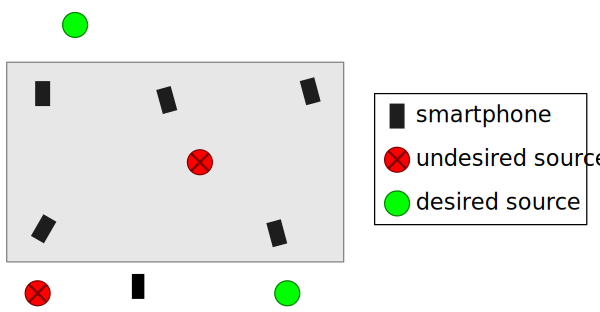
\includegraphics[width=0.6\textwidth]{afbeeldingen/goal_example.png}
	    \caption[Example conference calling system configuration]{An example of a conference calling system configuration}
	    \label{fig:goal}
\end{figure}

A conference call is a telephone call in which two or more parties, possibly consisting of more than one person, can simultaneously communicate.
Conference calls are frequently used in large companies because they allow parties to communicate efficiently without travelling to the same location.
They facilitate team meetings or other occasions in which employees at different locations want to communicate by telephone.

Many large companies currently make use of expensive equipment in specialized rooms.
These systems are often difficult to configure and even then sound quality can not be guaranteed.
Because the audio signals are recorded with one microphone, most of the time positioned at the centre of the table, there is a lot of noise and options for noise cancellation are limited.
A more accessible and convenient solution would be to only use the participants smartphones for such a system: a clear conference call could be held anywhere using a device nearly everyone already possesses.

Another application of such a system could be to help people with hearing aids to communicate.
Someone with a hearing aid has the same kind of problems as a modern conference call system: they cannot filter sounds from different directions, the sound volume is the same from every direction.
For example, when someone with a hearing aid is in a pub, it is very difficult for that person to concentrate on the voices of the people around him.
This is due to the voices of a person at for instance a table to his left being at the same volume as the voice of the person sitting in front of him.
This person could be helped if just a few people placed their smartphones on table and started an application, which connects to the hearing aid and dampens the distracting noises from the other tables at the pub.

An example of a possible conference calling system configuration is shown in Figure \ref{fig:goal}. Several smartphones are located on a table in a regular office environment. A number of desired audio sources (e.g. people speaking) and undesired noise sources (e.g. an air conditioning unit or background conversation) are located around the table. The smartphones are placed in an arbitrary but known positions and the locations of the desired and undesired sources are also assumed to be known. 

The smartphones are running a mobile application from which the sound data is acquired.
This data is then transmitted via a WiFi network and the signals are synchronised in order to make beamforming possible \cite{BAP:RoySjoerd}. 
Beamforming is a technique in the field of signal processing with the purpose to transmit or receive signals directionally \cite{VanVeen19884}.
The described system applies acoustic beamforming.
Hennecke and Fink \cite{hennecke2011towards} concluded that modern smartphones are suitable for acquiring audio signals as input for a beamforming algorithm.
The received signals from the smartphone microphones can be processed into one resulting audio stream.

These microphone signals can be used to amplify the desired signal and suppress background noise.
This is done by spatial filtering, using the given location information of the smartphone microphones and desired and noise sources.
There exist several acoustic beamforming algorithms, each having their own advantages and disadvantages \cite{BAP:ErikNiels}. 
Beamforming will be further explained in this thesis in Section \ref{ssec:background-beamforming}, as this thesis focuses on a three-dimensional directivity gain pattern to improve the result of a beamforming algorithm.
A directivity gain pattern, from now on referred to as \textit{directivity}, gives information about the directional gain of, for instance, a microphone.
The directional gain indicates how a signal of a certain frequency originating from a certain place is attenuated and delayed.

Research on the application of smartphone microphone directivity in a beamforming algorithm has been performed before \cite{Gaubitch2014}, but this research only describes the directivity in one plane and not for all directions.
Still, this research points out that including the two-dimensional microphone directivity in a beamforming algorithm considerably improves the results of the beamforming algorithm. 
It is thus plausible that a three-dimensional microphone directivity will enhance the performance of a beamforming algorithm even more. 
The aim of this thesis is to determine the three-dimensional directivity of a smartphone microphone.
This directivity will be implemented in a larger system to apply beamforming on audio signals recorded by smartphones. 
The directivity behaviour will be determined by examining the impulse response of the microphone for a variety of sample directions.

\begin{figure}[h!]
    \centering
    \includegraphics[width=0.8\textwidth]{afbeeldingen/blokschema4.png}
	\caption[The contribution of the directivity measurements]{The contribution of the directivity measurements in the whole system.}
	\label{fig:system}
\end{figure}

\section{Objective}
An overview of the whole system is shown in Figure \ref{fig:system}.
This thesis describes one of the three parts of the design to make a conference calling system as describe above possible.
The part concerning the smartphone array, including communication between smartphones and the computer, and the synchronisation of the audio signals is left to Bosma and Smeding \cite{BAP:RoySjoerd}.
The implementation of different beamforming algorithms and the quality comparison for these different algorithms was performed by Van Wijngaarden and Wouters \cite{BAP:ErikNiels}.

The green box marks the study of this thesis: determining the directivity gain pattern of a smartphone microphone and apply this directivity to a beamforming algorithm.
This thesis will describe the process of measurement, processing and displaying the data.
An important question that needs to be answered is how representative one measurement is for different settings of the smartphone and for different phones of the same type. 
For this project \nexus~ is used. Not much information is available about the microphones used in this smartphone or their directivities.
Therefore the directivities of the microphones will have to be determined by measurement, with as much accuracy as possible in the given time. 
The objectives for the function, as a part of the beamforming system, are specified more precisely in the schedule of requirements, in Appendix \ref{app:requirements}. 

%\FloatBarrier
\section{Thesis structure}
This thesis starts with the theoretical background of measuring microphone directivities in Chapter \ref{chap:background}.
Subsequently the available resources, measurement set-up and decisions made will be discussed in Chapter \ref{chap:measurements}.
The results of these measurements were not directly usable, but needed to be equalized to support the beamforming algorithm.
This process is described in Chapter \ref{chap:equalization}.
After this, the final results and a discussion of these results will be presented in Chapter \ref{chap:outcome} in Section \ref{sec:results} and Section \ref{sec:discussion} respectively.
Finally, a conclusion and our recommendations for future work are presented in \ref{chap:conclusion}. \\
Ethical considerations regarding the project are added in Appendix \ref{app:ethical}.

\section{Definitions and notation}
Throughout this thesis, there will be definitions and (mathematical) notation, which will be presented in advance.
If $x[n]$ is a discrete time signal, with N entries and $n=1,2,\ldots,N$, $\mathbf{x}$ is the vector notation of the signal and $X[\omega]$ ($\mathbf{X}$ in vector) is its discrete Fourier domain counterpart.
$\mathbb{N}_0$ denotes the set of natural numbers, with 0 includes: 0, 1, 2, 3,$\ldots$ and $\mathbb{N}$ denotes the set of natural numbers larger than 0: 1, 2, 3, 4,$\ldots$.
For matrices non-bold capitals will be used.
The convolution $c[n]$ of two signals $a[n]$ and $b[n]$ is written using an asterisk:
\begin{equation*}
c[n]=(a*b)[n].
\end{equation*}

For vector multiplication, assume two vectors $\mathbf{a}$ and $\mathbf{b}$, then its dot product or inner product $\mathbf{c}$ is written as:
\begin{equation*}
\mathbf{c}=\langle \mathbf{a},\mathbf{b}\rangle
\end{equation*}
and its cross product or vector product $\mathbf{d}$ written as:
\begin{equation*}
\mathbf{d}=\mathbf{a}\times\mathbf{b}.
\end{equation*}

For rounding the following signs are used:
$\lceil\bullet\rceil$
for rounding up and
$\lfloor\bullet\rfloor$
for rounding down.

Quantities in this thesis are often expressed on a logarithmic scale using decibel (dB) units.
Since the units in these thesis are field units (unless specified otherwise), the field unit form of the decibel scale is used:
\begin{equation*}
20\log_{10}|\bullet|.
\end{equation*}
From this follows the inverse of the dB-scale:
\begin{equation*}
10^{\dfrac{\bullet}{20}}.
\end{equation*}

The definitions of the spherical coordinate-system can be found in Figure \ref{fig:bol_def}.
The azimuth, $\theta$, is the angle between the projection of the vector pointing from the origin to the point on the $x,y$-plane and the $x$-axis.
The elevation, $\phi$, is the angle between the projection of the vector pointing from the origin to the point on the $x,z$-plane and the $z$-axis.
In Figure \ref{fig:def_nexus}, the definitions of the different sides of a smartphone are given.
The top of the smartphone, we will be called the listeningside, the bottom the speechside, the left side of the screen is the left side of the phone, the other side is the right side.
For specifying the orientation of the phone, the terms `screen up' and `screen down'  or `face up' and `face down' are also used.

If the phone is placed in the spherical coordinate system, the listeningside of the phone is pointing towards $(\phi,\theta)=(90^\circ,0^\circ)$.
Laying in the $(x,y)$-plane, with the screen face up towards the $+z$-direction.

The last thing to note is that all code for this thesis was written for \matlab~ Student R2014a. For some some of the hardware used in this thesis special drivers are needed, which can be found via the reference given when the hardware is mentioned.

\vspace{1in}

\begin{figure}[h]
\centering
\begin{subfigure}[t]{0.45\textwidth}
    \centering
    \includegraphics[width=\textwidth]{afbeeldingen/azel.jpeg}
    \caption{Definitions on a sphere, azimuth $\theta$, elevation $\phi$}
    \label{fig:bol_def}
\end{subfigure}~
\begin{subfigure}[t]{0.45\textwidth}
    \centering
    \includegraphics[width=\textwidth]{afbeeldingen/nexus_sides.jpg}
    \caption{Definitions of the different sides of the smartphone. Picture of {\nexus} used from \cite{nexus:figure}.}
    \label{fig:def_nexus}
\end{subfigure}
\caption[Definitions in this thesis]{Definitions used throughout this thesis.}
\label{fig:def}
\end{figure}